\documentclass[14pt,aspectratio=169,xcolor=dvipsnames]{beamer}
\usetheme{SimplePlus}
\usepackage{booktabs}
\usepackage{minted}

\title[short title]{Clase 4: I/O, interactividad}
\subtitle{}
\author[NA Barnafi] {Nicolás Alejandro Barnafi Wittwer}
\institute[UC|CMM] 
{
    Pontificia Universidad Católica de Chile \\
    Centro de Modelamiento Matemático
}

\titlegraphic{
    \vspace{-1.8cm}
    \begin{flushright}
      
\includegraphics[height=2.5cm]{../images/logos/puc.png} 
    \end{flushright}
}

\date{}
%\setbeamercovered{transparent}

\begin{document}
%%%%%%%%%%%%%%%%%%%%%%%%%%%%%%%%%%%%%%%%%%%%%%%%%%%%%%%
\begin{frame}
    \maketitle
\end{frame}
%%%%%%%%%%%%%%%%%%%%%%%%%%%%%%%%%%%%%%%%%%%%%%%%%%%%%%%
%%%%%%%%%%%%%%%%%%%%%%%%%%%%%%%%%%%%%%%%%%%%%%%%%%%%%%%
\section{I/O (Input/Output)}
%%%%%%%%%%%%%%%%%%%%%%%%%%%%%%%%%%%%%%%%%%%%%%%%%%%%%%%
%%%%%%%%%%%%%%%%%%%%%%%%%%%%%%%%%%%%%%%%%%%%%%%%%%%%%%%
\begin{frame}\frametitle{Motivación}
    \begin{itemize}
        \item El genoma human pesa $\approx$ 1Gb (película en def standard)
        \item El genoma del krill pesa $\approx$ 12Gb
        \item CPU procesa hasta 64 Kb a la vez
    \end{itemize}
    \hspace{2cm}
\includegraphics[height=4cm]{../images/vitruvio.jpg}
    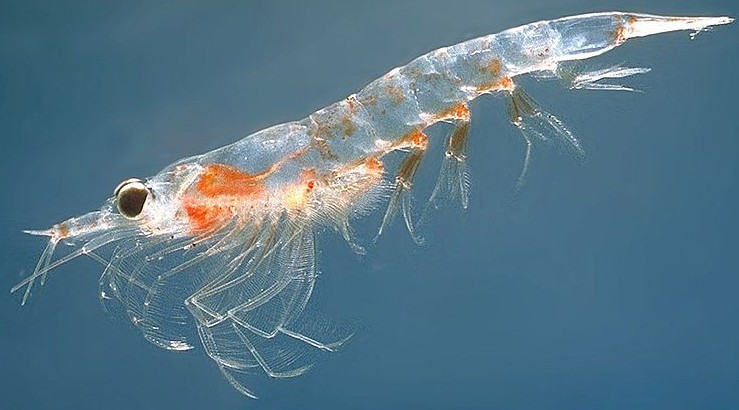
\includegraphics[height=4cm]{../images/krill.jpg}

\pause Necesitamos procesar datos sin cargar todo en memoria (\emph{streams})
\end{frame}
%%%%%%%%%%%%%%%%%%%%%%%%%%%%%%%%%%%%%%%%%%%%%%%%%%%%%%%
\begin{frame}[fragile]\frametitle{Lectura de archivos}
Archivo \texttt{pangramas.txt}:
    \begin{verbatim}
The quick brown fox jumps over the lazy dog
Extraño pan de col y kiwi se quemó bajo fugaz vaho
Ma la volpe col suo balzo ha raggiunto il quieto Fido
Törkylempijä vongahdus
    \end{verbatim}

    \begin{minted}{python}
    f = open("../archivos/pangrams.txt", "r") # (r)ead
    f.read() # o readline(), o readlines()
    f.close()
    \end{minted}
\end{frame}
%%%%%%%%%%%%%%%%%%%%%%%%%%%%%%%%%%%%%%%%%%%%%%%%%%%%%%%
\begin{frame}[fragile]\frametitle{Escritura}
    \begin{minted}{python}
    f = open("../archivos/pangrams.txt", "w") # (w)rite
    f.write() # o writelines()
    f.close()
    \end{minted}

*Es siempre importante \emph{cerrar} el archivo
\end{frame}
%%%%%%%%%%%%%%%%%%%%%%%%%%%%%%%%%%%%%%%%%%%%%%%%%%%%%%%
\begin{frame}[fragile]\frametitle{Uso común}
    Se usa contexto con {\color{purple}\texttt{with}} para cierre automático
    \begin{minted}{python}
    with  open("ejemplo.txt", "w") as f
        f.write("texto nuevo\n") 
    # fin de 'with'
    [...]
    \end{minted}
\end{frame}
%%%%%%%%%%%%%%%%%%%%%%%%%%%%%%%%%%%%%%%%%%%%%%%%%%%%%%%
\begin{frame}[fragile]\frametitle{Modos de lectura}
    \begin{itemize}
        \item 'r': Lee archivo, error si no existe
        \item 'w': Escribe en un archivo. Sobreescribe si existe
        \item 'x': Crea archivo, error si ya existe
        \item 'a': Agrega a archivo al final. Lo crea si no existe.

    \end{itemize}
    
    \vspace{1cm}
    \begin{minted}{python}
    modo = "w" # r|w|x|a
    with open("ejemplo.txt", modo) as f
        [...]
    \end{minted}
\end{frame}
%%%%%%%%%%%%%%%%%%%%%%%%%%%%%%%%%%%%%%%%%%%%%%%%%%%%%%%
\begin{frame}

\idea{Consola...}

\end{frame}
%%%%%%%%%%%%%%%%%%%%%%%%%%%%%%%%%%%%%%%%%%%%%%%%%%%%%%%
%%%%%%%%%%%%%%%%%%%%%%%%%%%%%%%%%%%%%%%%%%%%%%%%%%%%%%%
\section{Scripts interactivos}
%%%%%%%%%%%%%%%%%%%%%%%%%%%%%%%%%%%%%%%%%%%%%%%%%%%%%%%
%%%%%%%%%%%%%%%%%%%%%%%%%%%%%%%%%%%%%%%%%%%%%%%%%%%%%%%
\begin{frame}[fragile]\frametitle{Motivación}
    \begin{minted}{python}
    a = 2
    textfile = "../carpeta/archivo.txt"
    procesar(a, textfile)
    \end{minted}
    \begin{itemize}
        \item Poco portable
        \item Poco modular
        \item Ej: correr código para 1000 valores de 'a' en 15 archivos
    \end{itemize}

\pause \idea{Buscamos solución fuera del código}
\end{frame}
%%%%%%%%%%%%%%%%%%%%%%%%%%%%%%%%%%%%%%%%%%%%%%%%%%%%%%%
\begin{frame}[fragile]\frametitle{Input}
    Solución \#1: Frenar ejecución hasta que usuario entregue valor
    
    \begin{minted}{python}
    a = input("Ingrese valor de 'a': ")
    print(a, type(a))
    \end{minted}

    \vspace{1cm}
    El valor ingresado es un \code{str}
\end{frame}
%%%%%%%%%%%%%%%%%%%%%%%%%%%%%%%%%%%%%%%%%%%%%%%%%%%%%%%
\begin{frame}[fragile]\frametitle{Argv}
    Solución \#2: Usar parámetros de programa
    \begin{minted}{python}
    # programa.py
    from sys import argv
    name = argv[0]
    arg1 = argv[1]
    arg2 = argv[2]
    print("argv:", name, arg1, arg2)
    \end{minted}

    Luego en bash:
    \begin{minted}{bash}
    $ python programa.py 'hola' 42
    argv: programa.py hola 42
    \end{minted}
\end{frame}
%%%%%%%%%%%%%%%%%%%%%%%%%%%%%%%%%%%%%%%%%%%%%%%%%%%%%%%
\begin{frame}

\idea{Consola...}

\end{frame}
%%%%%%%%%%%%%%%%%%%%%%%%%%%%%%%%%%%%%%%%%%%%%%%%%%%%%%%
\begin{frame}\frametitle{Recap}
    \begin{itemize}
        \item Lectura a través de \emph{stream}
        \item Lectura de archivos con \code{open}
        \item Contexto con \code{with}
        \item Modos de lectura: \code{r},\code{w},\code{a}
        \item Vimos cómo hacer scripts interactivos
        \item \code{input} para esperar info del usuario
        \item \code{argv} para que el input sea parte del programa
    \end{itemize}
\end{frame}
%%%%%%%%%%%%%%%%%%%%%%%%%%%%%%%%%%%%%%%%%%%%%%%%%%%%%%%
\begin{frame}
    \maketitle
\end{frame}
%%%%%%%%%%%%%%%%%%%%%%%%%%%%%%%%%%%%%%%%%%%%%%%%%%%%%%%
\begin{frame}[fragile]\frametitle{Mini ejercicios}
    \begin{itemize}
        \item Cree un script que lea un archivo que tenga un número por fila y los sume
        \item Cree un programa que sume todos los números dados al programa: 
        \begin{minted}{bash}
    $ python programa.py 2 3 4 5  
    Los números suman 14
        \end{minted}

\idea{Para convertir un string a float, use \code{float(myString)}}
    \end{itemize}
\end{frame}
%%%%%%%%%%%%%%%%%%%%%%%%%%%%%%%%%%%%%%%%%%%%%%%%%%%%%%%
\end{document}
